% sample comment

% document type
\documentclass{beamer}
% settings and stuff
\usepackage{default}
\usetheme{Warsaw}
\definecolor{WOWIE}{RGB}{70,230,200} % these can be modified
\setbeamercolor{structure}{fg=WOWIE!90!black} % custom color
\usepackage{graphicx}
\graphicspath{ {"images"/} }
\usepackage[backend=bibtex]{biblatex}
\addbibresource{bibfile.bib}


% These packages will add fonts or commands that are useful
\usepackage{amsmath} % greek letters
\usepackage{soul,color} % these packages are used for edit command
\usepackage{amssymb} % cool math letter fonts

% customize formatted figure captions
\setbeamerfont{caption}{size=\tiny}
\setlength\abovecaptionskip{-5pt}
\setbeamertemplate{caption}{\raggedright\insertcaption\par}

% This is where we can make custom commands (not all commands are as bad as the first
% markup command named edit
\makeatletter
\newcommand\SoulColor{%
	\let\set@color\beamerorig@set@color
    \let\reset@color\beamerorig@reset@color}
\makeatother
\SoulColor
\newcommand{\edit}[1][!!!!!]{\textcolor{red}{\SoulColor\hl{#1}}} 
    
% stuff for math-related formatting
\theoremstyle{definition}
\newtheorem{defn}{Definition}
\newtheorem*{defn*}{Definition}
\theoremstyle{example}
\newtheorem{examp}{Example}
\theoremstyle{conjecture}
\newtheorem{conj}{Conjecture}
% convenient absolute value 
%\DeclarePairedDelimiter\abs{\lvert}{\rvert}
%\makeatletter
%\let\oldabs\abs
%\def\abs{\@ifstar{\oldabs}{\oldabs*}} % star prevents auto resize
%\makeatother
\def\code#1{\texttt{#1}} % JA: for inline code
% convenient space shorthands
\newcommand{\Rone}{\mathbb{R}}
\newcommand{\Rtwo}{\mathbb{R}^{2}}
\newcommand{\Rthree}{\mathbb{R}^{3}}
\newcommand{\Natnums}{\mathbb{N}}
\newcommand{\Integers}{\mathbb{Z}}
% big O notation
\newcommand{\Obig}{\mathcal{O}}
\newcommand{\bigslant}[2]{{\raisebox{.2em}{$#1$}\left/\raisebox{-.2em}{$#2$}\right.}} % quotient spaces
% complexity theory shortcuts
\newcommand{\Time}{\text{\textbf{TIME}}}
\newcommand{\Space}{\text{\textbf{SPACE}}}
\newcommand{\pspace}{\text{\textbf{PSPACE}}}
\newcommand{\np}{\text{\textbf{NP}}}
\newcommand{\p}{\text{\textbf{P}}}
\newcommand{\exptime}{\text{\textbf{EXPTIME}}}
\newcommand{\expspace}{\text{\textbf{EXPSPACE}}}
% convenient superscripts
\newcommand{\Th}{^{\text{th}}}
\newcommand{\St}{^{\text{st}}}


% This is where the document begins
\begin{document}

\title{Topological Data Analysis on Libraries.io Data}
\author{Brian Friend, Jacob Miller, Jonathan Anderson, Kaixiang Wang}
\date{\today}

% first slide will be a title page
\begin{frame}
\maketitle
\end{frame}

% second slide will be table of contents
\begin{frame}{Contents}
\small{
\tableofcontents
}
\end{frame}

% Sections will be displayed in table of contents
\section{Background}
\label{sc.background}
% subsection on the data source
\subsection{The Data}
\label{subsc.datasource}
\begin{frame}{What data?}
Package Managers \& libraries.io:
  \begin{itemize}
  	\item project goal: how are open-source projects connected?
    \item libraries.io monitors millions of open-source project libraries 
    	  and dozens of package managers
    \item keeps track of dependencies, version information, etc.
    \item libraries.io's main file had millions of lines of this information
    \item we looked at subset of that data:\
          \code{CPAN}, \code{CRAN}, \code{Brew}, \code{Dub}
  \end{itemize}
\end{frame}

% subsection TDA -- including graph theory and persistent homology
\subsection{Topological Data Analysis}
\label{subsc.tdabackground}
\begin{frame}
\textbf{TDA}
  \begin{itemize}
    \item Starting out with the high dimensional point cloud
    \item unknown lower-dimensional structure
    \item TDA is a collection of methods for "teasing out" topological structure
  \end{itemize}
\end{frame}

\begin{frame}
\begin{defn}
\textbf{Topology} is the study of spaces and the features that describe spaces.
\end{defn}
\vfill
\begin{defn}
\textbf{Topological Data Analysis (TDA)} is the practice of analyzing the spatial properties of data sets.
\end{defn}
\end{frame}

\begin{frame}{Spatial Properties}
\begin{columns}
\begin{column}{.5\textwidth}
Properties include the following:\\
\begin{itemize}
\item \vphantom{How many relations are there between data points}Connectedness
\item \vphantom{How can data be categorized}How a space can be separated
\item \vphantom{How do the dimensions of data interact}The types of holes found in a space
\end{itemize}
\end{column}
\begin{column}{.5\textwidth}
What this means in data terms:\\
\begin{itemize}
\item \vphantom{Connectedness}How many relations are there between data points
\item How can data be categorized\vphantom{How a space can be separated}
\item \vphantom{The types of holes found in a space}How do the dimensions of data interact
\end{itemize}
\end{column}
\end{columns}
\end{frame}

% Section on our methods
\section{Methods}
\label{sc.methods}
\subsection{Data Storage}
\label{subsc.storage}
\begin{frame}{Initial Data Set}
Accessing the data:
\begin{itemize}
  \item Reproducibility using centralized location for data:\\
  https://libraries.io/data
  \item Downsides of Libraries.io's API:\\
  formatting, readability, etc.
  \item Benefits of downloading it ourselves:\\
  		flexibility, managing data size, filtering data
\end{itemize}
\end{frame}

\subsection{Shell Scripts}
\label{subsc.scripts}
\begin{frame}{Extracting Relevant Data}
Size \& Filtering:
\begin{itemize}
  \item Size problems:\\
  \begin{tabbing} % This is to align the file sizes
  \emph{compressed} data was \quad \=5.9\ \= GB,\\
  and uncompressed was \>33\ \> GB % Great to safe the colorful explanation for speaking
  \end{tabbing}
  \item Focused on ``\code{dependencies.csv}''
  \item Python wrapper \code{process.py} separates data into different files % Say: calls egrep
  \item Scripts for stripping out redundant, 
  		missing information % for Cytoscape
\end{itemize}
\end{frame}

\subsection{Software Exploration}
\label{subsc.software}
\begin{frame}
Problems with non-TDA software:
\begin{itemize}
  \item Limitations of \code{Python}% This is what is mentioned during talking: great for extraction and treating data, but quickly hobbled by speed, memory limitations in 32-bit mode, and inflexible graphing
  \item Poor \code{R} documentation% again save for speaking: is another personal favorite, but it's (this is non-TDA) TDA packages aren't mature or friendly, and graphics are even more of a mess.
  \item Summary of issues:\\
 	\begin{itemize}
	   \item maturity of tools
       \item speed
       \item memory usage
       \item graphical flexibility
   	   \item monitering execution
 	\end{itemize}
\end{itemize}
\end{frame}

\subsection{Cytoscape}
\label{subsc.cytoscape}
\begin{frame}
Explanation \& Justification for Cytoscape:
\begin{itemize}
  \item previous software problems all largely solved by using CytoScape
  \item maturity: online community, documentation that doesn't require a PhD
  \item memory usage: larger graphs require more memory but Cytoscape actually lets you use it
  \item graphics: beautiful and extremely elegant graphing utilities
  \item micromanagement: change data representation on the fly
  \item Conclusion: 
  		using already developed software allowed us to get 
        to exploring dependency information without reinventing the wheel
\end{itemize}
\end{frame}

\subsection{TDA for R}
\label{subsc.r}
\begin{frame}
For comparison's sake and for quantifying relationships, 
we're in the rough stages of integrating \code{R}'s TDA package..
\begin{itemize}
  \item https://cran.r-project.org/web/packages/TDA/vignettes/article.pdf
  \item ``provides topological information about the underlying
space, such as the distance function, the distance to a measure, the kNN density estima-
tor, the kernel density estimator, and the kernel distance.  The salient topological features
of the sublevel sets (or superlevel sets) of these functions can be quantified with persistent
homology.''
\end{itemize}
\end{frame}

% Section on our analysis
\section{Analysis}
\label{sc.analysis}
% Subsection on traditional tda
\subsection{Traditional TDA}
\label{subsc.tradtda}
% \begin{frame}{Graph Theoretic Results}
% Explain the topological data analytics are a results of cytoscape with pretty pictures.\\
% Possibly include images like this:
% \begin{figure}
% 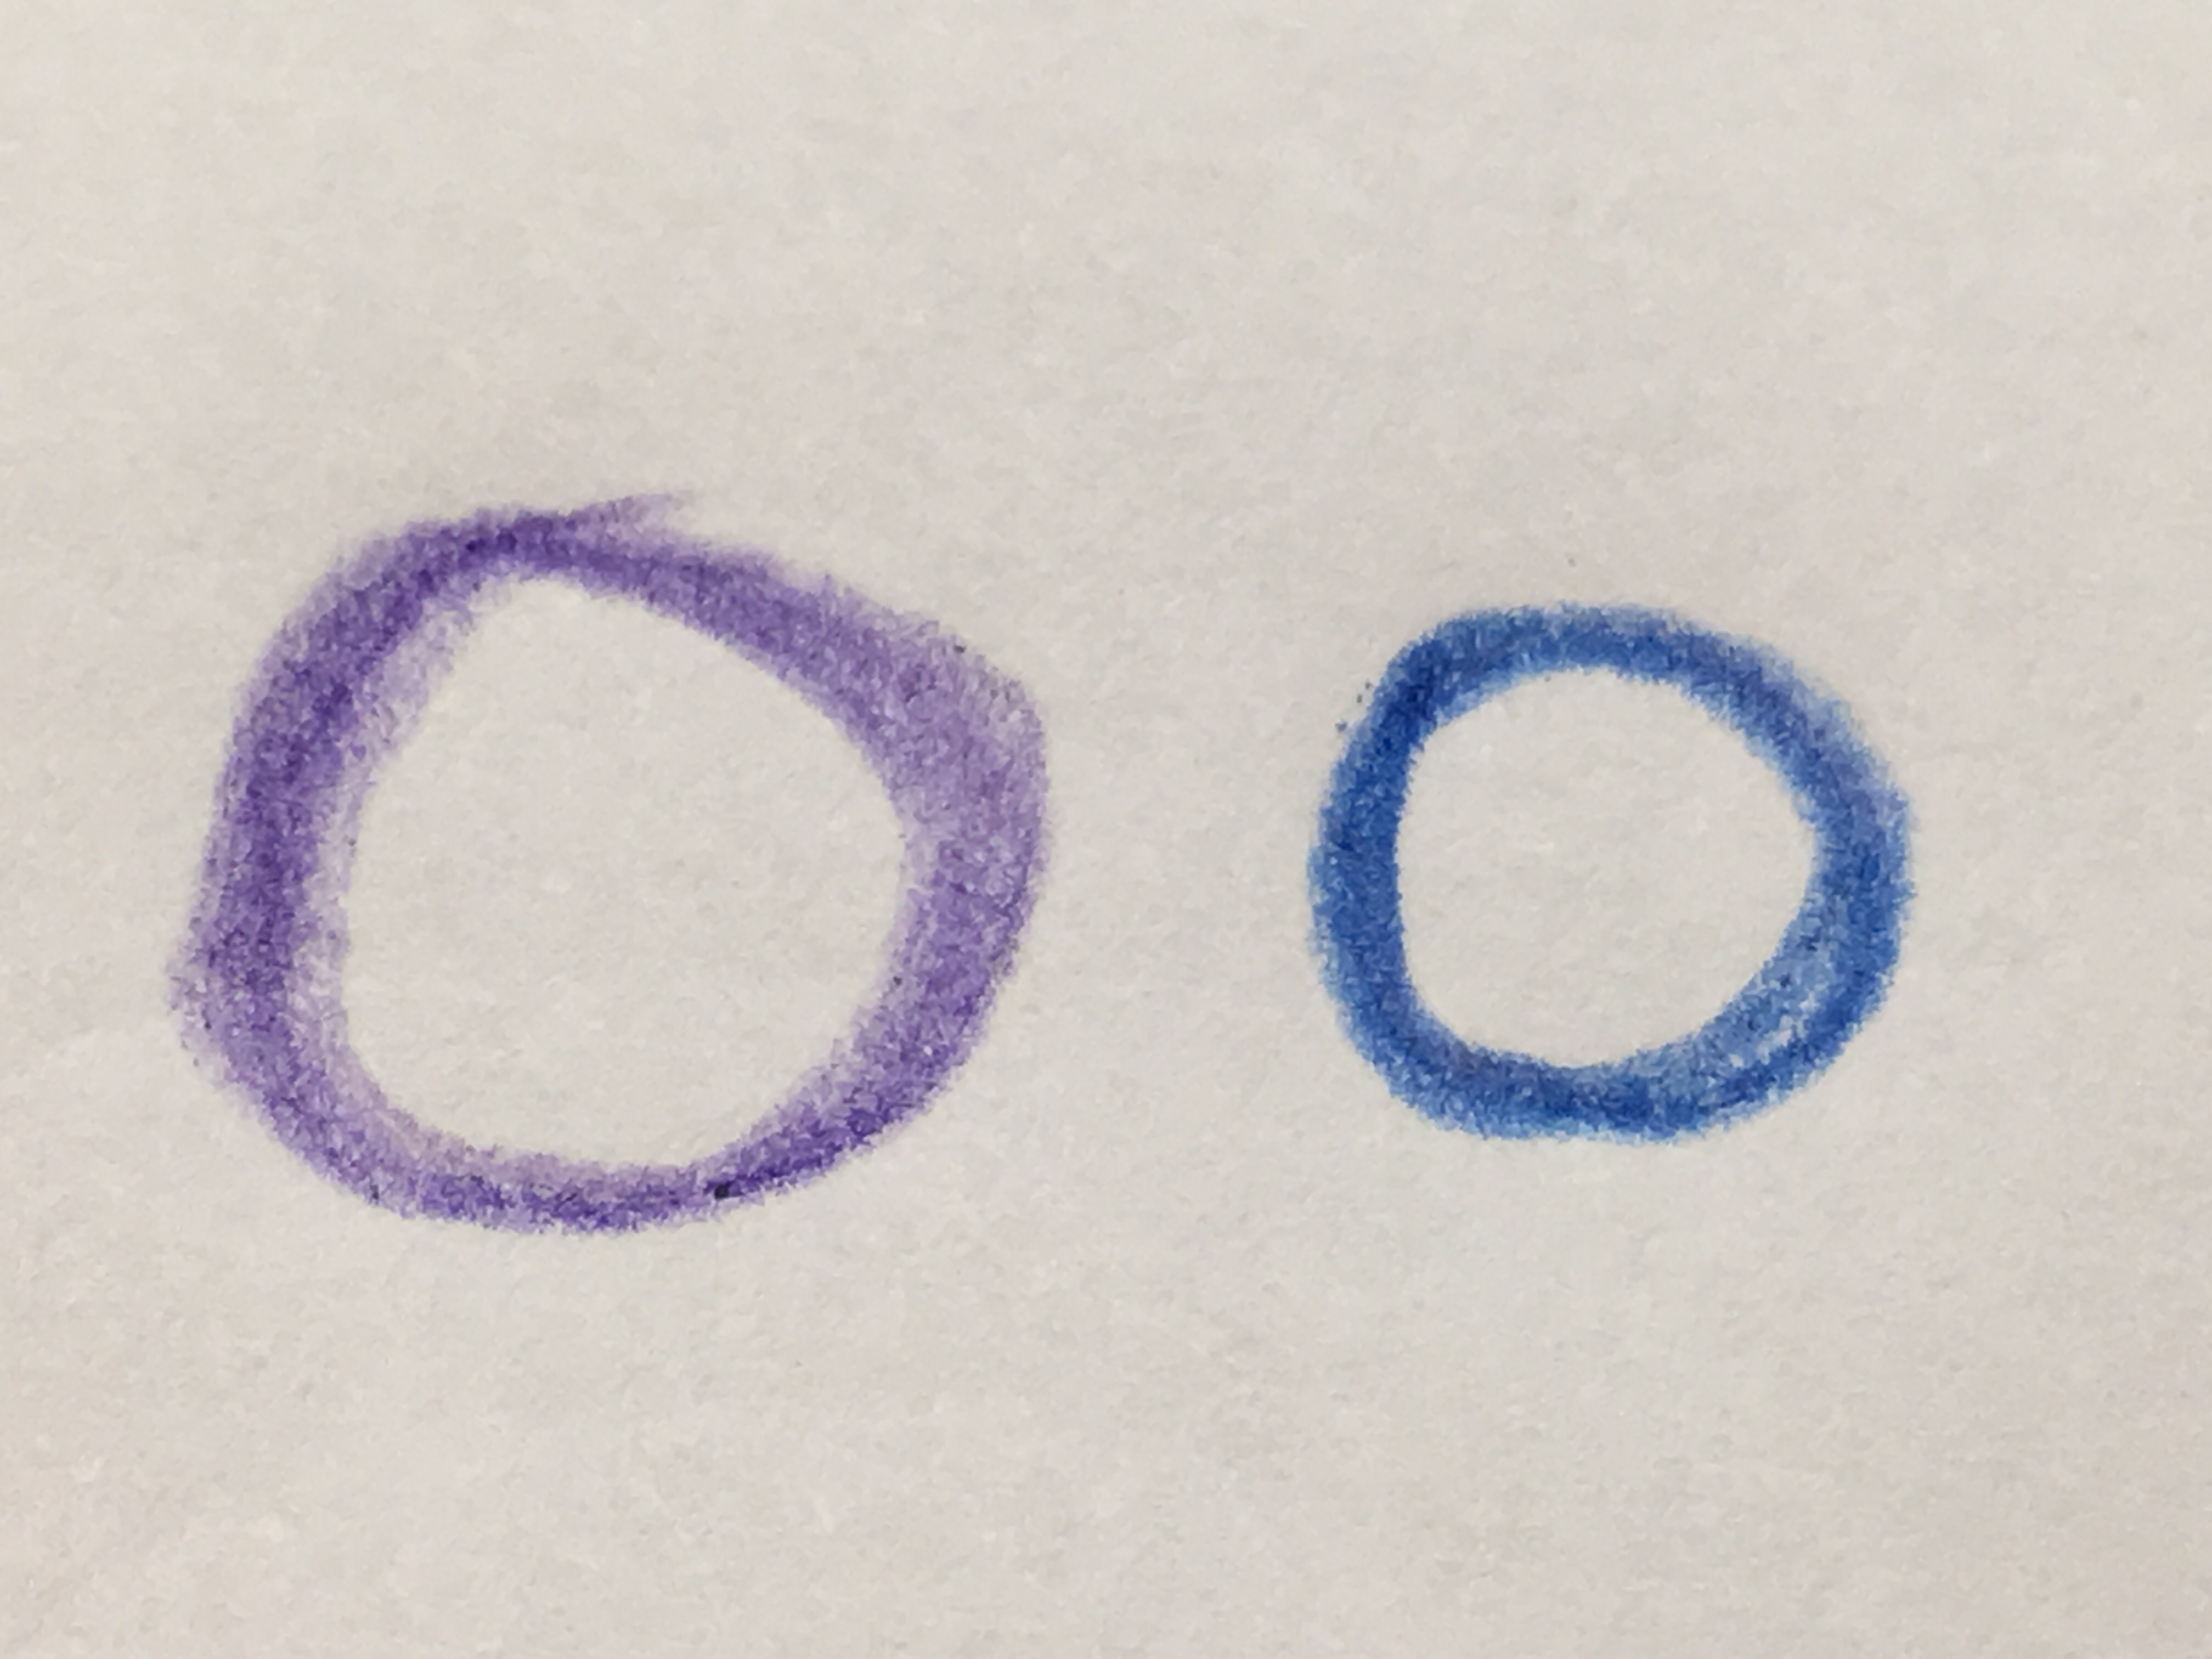
\includegraphics[width=5cm, height=4cm]{unlinked_circles}
% \caption{This image is from my masters thesis.}
% \end{figure}
% \end{frame}

% \begin{frame}
% \begin{defn}
% A \textbf{cat} is a fury animal.
% \end{defn}
% \end{frame}

\begin{frame}
Graph Analysis is essential for TDA
	\begin{itemize}
    	\item Graph is a direct virtual way to help people build understanding to a data structure.
	\end{itemize}
\begin{figure}
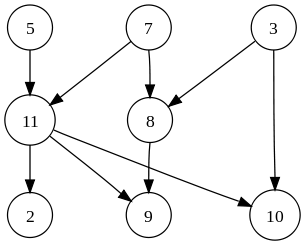
\includegraphics[width=5cm, height=4cm]{Graph_example}
\end{figure}
\end{frame}

\begin{frame}
There are important parameters to help people analysis the graph.\\
\begin{itemize}
    \item Vertices % spelling is correct
    \item Edges
    \item Orientation % more meaningful word for the sake of asymmetric graphs
\end{itemize}
\end{frame}

\begin{frame}
Example graphs from sample Data Dub.csv
\begin{figure}
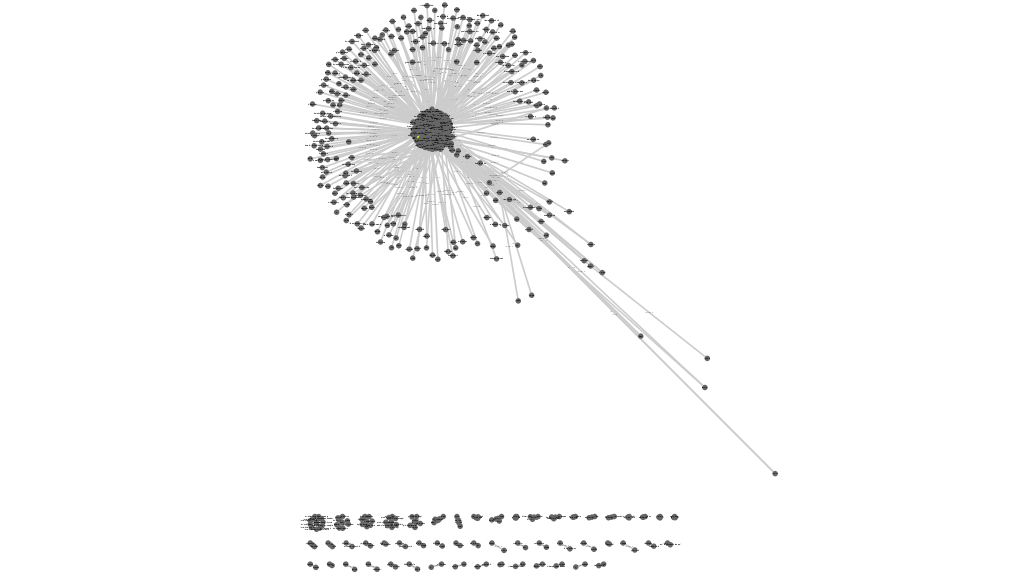
\includegraphics[width=10cm, height=5cm]{Dub_csv_GrayNode}
\end{figure}
\end{frame}

\begin{frame}
Example graphs from sample Data Dub.csv
\begin{figure}
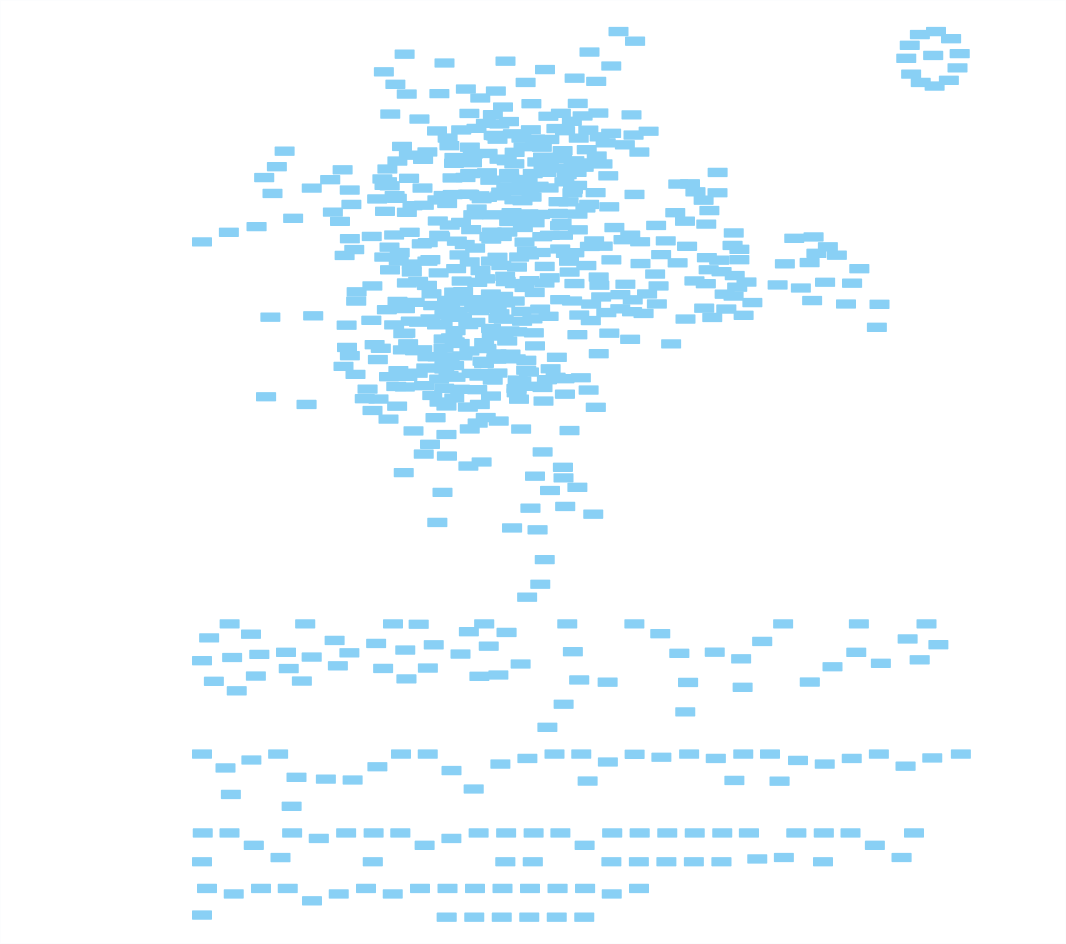
\includegraphics[width=6cm, height=5cm]{Dub-general-idea}
\end{figure}
\end{frame}

% \begin{frame}
% This slide will demonstrate how a citation works in beamer.\\
% \vfill
% According to Roger, rain is wet \cite{lang_algebra_2002}
% \end{frame}

% % Subsection on new TDA
% \subsection{Persistent Homology}
% \label{subsc.newtda}
% \begin{frame}
% Explain results of TDA tools with R. I will probably add this later if we have time.
% \end{frame}

% % Section for Discussion/conclusion
% \section{Discussion}
% \label{sc.discussion}
% \begin{frame}
% discuss results here\\
% \vfill
% \begin{columns}
% \begin{column}{.5\textwidth}
% This is on the left hand side
% \end{column}
% \begin{column}{.5\textwidth}
% \begin{itemize}
% \item Test
% \item this
% \end{itemize}
% \end{column}
% \end{columns}
% \end{frame}

% % Bibliography
% \label{sc.references}
% \begin{frame}[t,allowframebreaks]{References}
% 	\printbibliography
% \end{frame}

\end{document}
